\chapter{Evaluation}\label{sec:evaluation}


% \begin{blockquote}
%     \paragraph{Intent:} Performance evaluation 
%     Structure:
%     \begin{description}

%         \item[Experimental setup] Optimization problems types, evaluation assumption and budget, repetition

%         \item[Benhmark 1] Default Tutor-model(portfolio, thresholds) on plethora types of multiobjective problems
%         \begin{enumerate}
%             \item default Tutor-model parameters
%             \item surrogate portfolio items
%             \item Baseline: MOEA
%         \end{enumerate}

%         \item[Benhmark 2] Parameter selection of Tutor-model with the dynamic sampling plan
%         \begin{enumerate}
%             \item Parameters: prediction count, train/test split, stacking solutions. thresholds(x2), solver
%             \item Subset of problems
%             \item Baseline: Static vs Dynamic. Parameters tune
%         \end{enumerate} 

%         \item[Benhmark 3] Many-objective optimization. Objectives>10
%         \begin{enumerate}
%             \item Static Heterogeneous compositional surrogate vs. Homogeneous compositional surrogate
%             \item Base line: MOEA or Random
%         \end{enumerate}

%         \item[Discussion] Results interpretation
%     \end{description}
% \end{blockquote}


In this chapter, we compare over our developed approach with state-of-the-art strategies: evolutionary algorithms and static compound model-based optimization.

% ? MOEA is called globally convergent if the produced, non-dominated population converges to the true Pareto front while the number of generations goes to infinity.


% --------------------------------------------------------------------------------------------
% ------------------------------------------------     Experimental setup     
% --------------------------------------------------------------------------------------------
\section{Experimental setup}
    We introduce a description of selected optimization problems and general parameters for analysis.

    % ---------------------------------     Optimization problems
    \subsection{Optimization problems}
    Numerous types of problems need to be considered to reduce the bias of the results. For comparison was selected several comprehensive synthetic benchmark suites. All of them are scalable in parameter space and some are scalable in objective space. The problems are designed so that a meaningful comparison can be obtained for optimization techniques. All cases are minimization problems.

    According to \cite{WFGref}, the following properties characterize the optimization problems:
    \begin{itemize}
        \item \emph{Modality} is a property of the objective surface. Test problems are either unimodal with one global optimum or multimodal with several local optima. Multimodal problems are more complicated than unimodal and more similar to real-world scenarios (Figure: \ref{fig:multi_modal_zdt4}). A deceptive objective function has a special kind of multimodality that have at least two optima — a true optimum and a deceptive optimum — but the majority of the search space must favor the deceptive optimum \cite{Deb99}.
        \item A \emph{geometry} of the Pareto optimal front can be convex, linear, concave, mixed, degenerate, disconnected, or some combination of the former. It directly influences the algorithm's performance. 
        \item A \emph{bias} of landscape transformations impacts the search process by biasing the fitness landscape. This property means that uniformly distributed parameters are responded to a bias area in objective space. This type of problem could be challenging if the bias region is far away from the Pareto-optimal front (Figure \ref{fig:bias_area_wfg1}).
        \item \emph{Many-to-one} fitness mapping means that different parameter vectors could produce the same objective vector. This property makes the search more difficult to optimizers because most solutions produce the same result.
        \item \emph{Not separability } of the problem means that it can not be solved if consider it as separate optimization problems for each objective.
    \end{itemize}

    \begin{figure}
        \centering
        \begin{subfigure}{\textwidth}
            \begin{subfigure}{0.64\textwidth}
                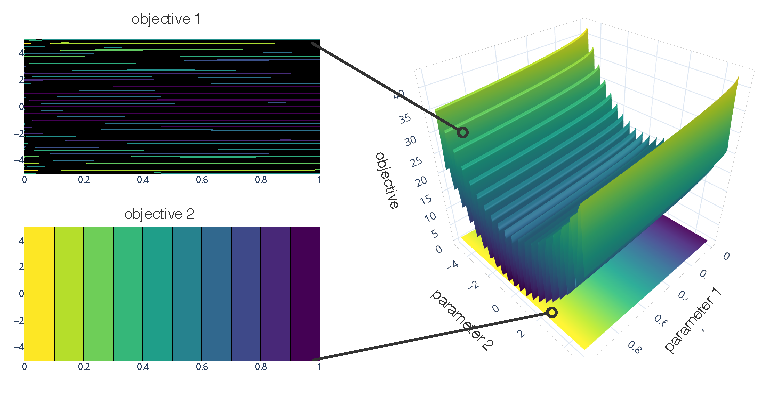
\includegraphics[width=\textwidth]{content/images/utility/multi_modal_zdt4}
                \caption{}
                \label{fig:multi_modal_zdt4}
            \end{subfigure} 
            \begin{subfigure}{0.35\textwidth}
                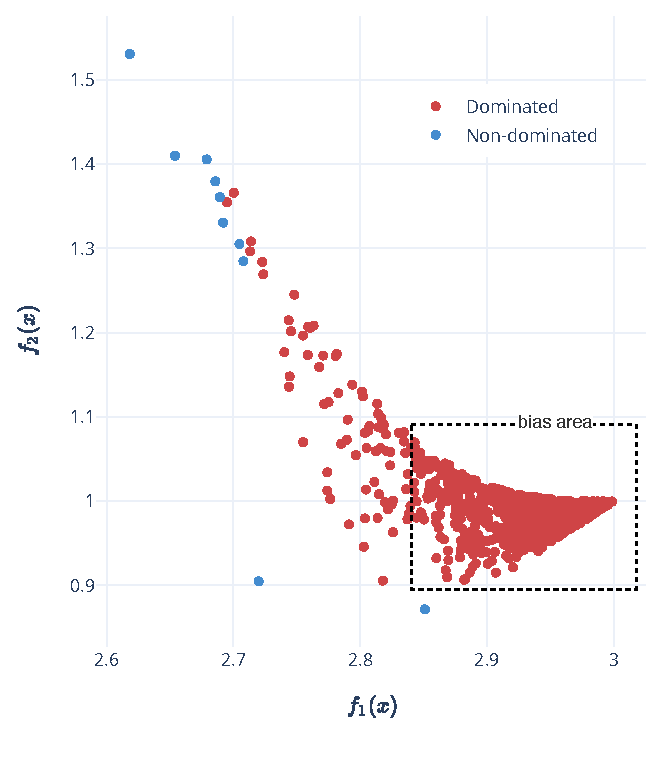
\includegraphics[width=\textwidth]{content/images/utility/bias_area_wfg1}
                \caption{}
                \label{fig:bias_area_wfg1}
            \end{subfigure} 
        \end{subfigure} 
        \caption[Example of unimodal, multimodal and bias problems]{\textbf{(a)} Example of ZDT4 problem landscapes with multimodal (\#1) and unimodal objectives (\#2). \textbf{(b)} Example of bias landscape in WFG1 problem. Note how, in this example, the objective vectors are denser far away from Pareto optimal solutions.}
        \label{fig:changing_models}    
    \end{figure}

    % ! [===    Many-to-one, bias, Modality, geometry  ===]
        % -----------------------------  ZDT      
        \paragraph{ZDT}\cite{ZitzlerDT00} is a test suite that consists of a set of two-objective problems and takes its name from its authors Zitzler, Deb and Thiele. In their paper the authors propose a set of 6 different scalable problems all originating from a well thought combination of functions allowing, by construction, to measure the distance of any point to the Pareto front. Each test function involves a particular feature that is known to cause difficulties in the evolutionary optimization process, mainly in converging to the Pareto-optimal front.
        For the evaluation we selected the following problems:
        \begin{itemize}
            \item ZDT1 has a convex Pareto-optimal front.
            \item ZDT2 has a non-convex Pareto-optimal front.
            \item ZDT3 adds a discreteness feature to the front. Its Pareto-optimal front consists of several noncontiguous convex parts. The introduction of a sine function in this objective function causes discontinuities in the Pareto-optimal front, but not in the parameter space.
            \item ZDT4 has 21 local Pareto-optimal fronts and therefore is highly multi-modal. It is also called a \textit{multifrontal} problem.
            \item ZDT6 has a non-uniform search space: the Pareto-optimal solutions are non-uniformly distributed along the global Pareto front, and also the density of the solutions is the lowest near the Pareto-optimal front and the highest away from the front.
        \end{itemize}


        % -----------------------------   DTLZ
        \paragraph{DTLZ}\cite{DebTLZ05} is an extensive test suite that takes its name from its authors Deb, Thiele, Laumanns and Zitzler. It was conceived for the multi-objective problems with scalable fitness and objective dimensions.  All problems in this test suite are box-constrained continuous n-dimensional multi-objective problems, scalable in fitness dimension. 
        \begin{itemize}
            \item DTLZ1  is one of the most difficult test problems in this test set. DTLZ1 has flat landscape regions, and the optimal Pareto front lies on a linear hyperplane. 
            \item DTLZ2 is a unimodal problem with the concave Pareto front.
            \item DTLZ3 is a multimodal problem with the concave Pareto front. DTLZ3 is upposed to be harder to converge towards the optimal Pareto front than DTLZ2.
            \item DTLZ4 is a unimodal problem with a bias to a dense area of solutions.
            \item DTLZ5 has a bias for solutions close to this Pareto-optimal curve. This problem may be easy for an algorithm to solve. Because of its simplicity, it is recommended to use with a higher number of objectives.
            \item DTLZ6 is more challenging version of the DTLZ5 problem with a non-linear distance function $g()$, which makes it harder to converge to against the Pareto front.
            \item DTLZ7 is a unimodal problem for the first objective and multimodal for the rest of the objectives. This problem has the disconnected Pareto-optimal front, which increases the likelihood that an \gls{ea} could fail to find all optimal regions.
        \end{itemize}

        % ------------------------------    WFG
        \paragraph{WFG}\cite{WFGref} test suite was designed to outperform the functionalities of previously implemented test suites. Essential improvements have been achieved in a majority of problems. Also, non-separable, deceptive, a mixed shape Pareto front problem are included. The WFG test suite was introduced by Simon Huband, Luigi Barone, Lyndon While, and Phil Hingston. 
        The test set includes the following problems:
        \begin{itemize}
            \item WFG1 is a unimodal problem with a convex and mixed Pareto front geometry. 
            \item WFG2 is a non-separable and unimodal problem with a convex and disconnected Pareto front geometry.
            \item WFG3 is a non-separable, unimodal problem in all its objectives except for the last one, which is multimodal.
            \item WFG4 is a multimodal problem with a concave Pareto front geometry. The multimodality of this problem has a landscape with large hills that make it more complicated for optimization.
            \item WFG5 is a separable problem with a deceptive landscape and a concave Pareto front geometry.
            \item WFG6 is the non-separable and unimodal problem. Its Pareto front geometry is concave. 
            \item WFG7 is a separable and unimodal problem with a concave Pareto front geometry. WFG7 together with the WFG1 are the only problems that are both separable and unimodal.
            \item WFG8 is a non-separable and unimodal problem with a concave Pareto front geometry.
            \item WFG9 is a multimodal, deceptive and non-separable problem with a concave Pareto optimal geometry. Similar to WFG6, the non-separable reduction of this problem makes it more complicated than that of WFG2 and WFG3.
        \end{itemize}



     The first benchmark presented a subset of the problems listed in Table \ref{bench_problems}. They have a wide range of properties which should give a notion of how the optimization strategy works. The results for all other problems are given in the appendix.
    % ==== multi-objective test problems
    \begin{table}[]
        \centering
        \resizebox{\textwidth}{!}{%
            \begin{tabular}{@{}cccccc@{}}
            \toprule
            \multirow{2}{*}{\textbf{Problem}} &
            \multirow{2}{*}{\textbf{Objective}} &
            \multirow{2}{*}{\textbf{Modality}} &
            \multirow{2}{*}{\textbf{Geometry}} &
            \multicolumn{2}{c}{\textbf{Landscape}} \\ \cmidrule(l){5-6}
                        &                 &                      &               & \textbf{Bias}    & \textbf{\begin{tabular}[c]{@{}c@{}}Many-to-one \\ mappings\end{tabular}} \\ \midrule
            \textbf{ZDT4}  & bi-objective    & unimodal, multimodal & convex        & -                & -                                                                        \\
            \textbf{ZDT6}  & bi-objective    & multimodal           & concave       & +                & +                                                                        \\
            \textbf{DTLZ4} & multi-objective & unimodal             & concave       & +                & +                                                                        \\
            \textbf{WFG1}  & multi-objective & unimodal             & convex, mixed & polynomial, flat & +                                                                        \\
            \textbf{WFG4}  & multi-objective & multimodal           & concave       & -                & +                                                                       \\ \bottomrule
            \end{tabular}%
        }
        \caption{Selected multi-objective test problems}
        \label{bench_problems}
    \end{table}


    % ---------------------------------     Optimization search
    \subsection{Optimization search}
    In this thesis, we do not perform an explicit parameter tuning for optimization algorithms. While multiple optimization algorithms could be applied, we selected \glspl{moea} as default optimization techniques for the surrogate models. The advantage of \gls{ea} is that it could be easily modified and it could operate on a set of solutions candidates, that are well-fitted to approximate the Pareto front. Also, \glspl{ea} can estimate highly complex problems in various use-cases. In this thesis, we used two types of \gls{ea}:

    \begin{enumerate}
        \item The popular evolutionary multi-objective algorithm \emph{NSGA2} \cite{DebAPM00}. We chose this algorithm as it popularity in \gls{moo}.  In all cases default parameters were used (population size = 100, crossover probability=0.95, distribution index for crossover=10.0, mutation probability=0.01, distribution index for mutation=50.0)\cite{francesco_biscani_2019}.
        \item As an alternative MOEA algorithm for optimization, we define \emph{MOEA-Ctrl} that combines MOEA/D \cite{ZhangL07} and NSGA2 algorithms. The characteristic of such an optimization process based on a common solutions population for both algorithms. Our intuition behind this choice is the following: NSGA2 gives stable results with well-distributed points on the Pareto front while MOEA/D has great exploration quality with low generation count. The combination of this algorithm should gain a better trade-off in exploration and exploitation in contrast to individual algorithms application.  
    \end{enumerate}

    % ---------------------------------    Portfolio
    \subsection{Surrogate portfolio}
    % The most popular and perspective models were selected for a default surrogate portfolio. All of them have benefits and drawbacks that depend on a particular use case. From multi-objective models, there is \emph{Gaussian Process Regressor} that commonly used in the Bayesian optimization. For this type of model should be specified by the prior's covariance. It is defined by passing a kernel object, the hyperparameters of which are optimized during extrapolations of the samples. The kernel for this benchmark is selected from the GPML\cite{RasmussenN10} and illustrate a complex kernel design. The Gaussian Process Regressor with this kernel was used to extrapolate the $CO_2$ concentration as a function of the time $t$. The kernel consists of several components that calibrate to represent a long term, periodic and medium components. Even though this kernel is from another domain, it does give good extrapolation quality for the regression model. Unfortunately, the build time is significant and grows with samples size and dimensionality.

    % Three models were selected for composite surrogates which give $3^{obj}$ possible surrogate combinations: 
    % \begin{itemize}
    %     \item Support Vector Regression (SVR) model with RBF kernel. SVR uses the same principles as the SVM for classification with the main idea is to minimize error and to individualize the hyperplane which maximizes the margin. With a motivation to extend the SVR to non-linear data, the kernel function transforms the data into a higher dimensional feature space that could be linearly separate.
    %     \item Multi-layer Perceptron regressor (MLPRegressor) with three hidden layers. A neural network is a popular and influential approach to approximate the functions landscape.
    %     \item Gradient Boosting Regressor that uses an ensemble decision tree regressors to produce a single model. Building process goes iteratively, at each step, a new tree is trained against the negative gradient of the loss function, that improve results in the previous step. This method accurate, and it applies to a variety of domain-problem.
    % \end{itemize}

    Based on our awareness, we selected the most popular models for a default surrogate portfolio.
    \begin{enumerate}
        \item \textbf{Gaussian Process Regressor} it is a multi-objective surrogate model that commonly used in the Bayesian optimization. For this type of model, the initialization should be specified by passing a kernel object, the hyperparameters of which are optimized during extrapolations of the samples.  The kernel for benchmarks is selected from the GPML\cite{RasmussenN10}. Even though this kernel is from another domain, it does give good extrapolation quality for the regression model. Unfortunately, the build time is significant and grows with samples size and dimensionality.
        \item \textbf{Support Vector Regression (SVR)} single-objective model with RBF kernel. Based on [cite] RBF and SVR are preferred for high dimensional problems.
        \item \textbf{Multi-layer Perceptron regressor (MLPRegressor)} A neural network is a popular and influential approach to approximate the functions landscape \cite{KOURAKOS201313}.
        \item \textbf{Gradient Boosting Regressor} is a single-objective model that uses an ensemble decision tree regressors to produce a single model.
    \end{enumerate}
    
    As a result, for bi-objective problems, there are no more than ten possible surrogate hypotheses (including multi-objective Gaussian Process Regressor). For a benchmark purpose, at each optimization round the surrogate portfolio does not change. 

    % ---------------------------------    Benchmark baseline
    \subsection{Benchmark baseline}
    We compare our approach (TutorM) with Hypermapper 2.0\cite{nardi2019practical} that was in Chapter~\ref{sec:related}. This toolbox focuses on multi-objective parameter tuning with various types of parameters. Hypermapper uses several randomized random forest models, one for each objective. The general idea is to scalarize several surrogate models to single-objective criteria and to optimize it as a single-objective problem. Besides, a Bayesian model is used to assist the search. Hypermapper was successfully used in autotuning computer vision applications and database optimization. Since the sample size is not specified, we have selected it as the default population size for the MOEA algorithm (100 points).

    NSGA 2 was chosen as it is one of the most well-known evolutionary algorithms \cite{RamirezRV19}. It is a suitable reference point to compare other approaches. In benchmarks, we evaluate two identical versions of the algorithm but with a different budget for evaluation:
        \begin{itemize}
            \item Small evaluation budget (1k) and used as a competing algorithm
            \item Large evaluation budget (10k and 50k) and used as a baseline
        \end{itemize}



    % NSGA 2 was chosen as the benchmark baseline, as it is one of the most well-known algorithm \cite{RamirezRV19}. It is a suitable reference point to compare other approaches. The results of budget-limited optimization algorithms should be closer to those results obtained from NSGA2 with a much larger budget. Budget means the available number of real function evaluations.

% --------------------------------------------------------------------------------------------
% ---------------------       Benchmark 1: Model-tutor: Portfolio with compositional surrogates 
% --------------------------------------------------------------------------------------------
\section{Benchmark 1: Portfolio with compositional surrogates. Dynamic sampling plan. [RQ1, RQ2]}
    In this benchmark, the developed approach(TutorM) was compared is related approaches in solving all three sets of problems (ZDT, DTLZ, WFG) for 2 objectives and 2(3) parameters. The TutorM includes all features such as dynamic compositional models, surrogate portfolio and validation. 
    The solution quality was evaluated by the following metrics: hypervolume, p-distance, spacing and number of available non-dominant solutions (ndf size)(Chapter ~\ref{sec:related}). The presented results obtained as the average value after five repetitions.

    % -------------------------------------------------------- One case
    \subsection*{One case studies: ZDT6}
    We start by comparing the runtime performance of the approaches. Let's consider runtime optimization for ZDT6 problem. On Figure \ref{fig:zdt6_dist} is shown optimization progress with an average distance to the Pareto front.  It could be notest that TutorM considerably outperforms NSGA2 and Hypermapper 2.0 right from the start of their optimization process. Our algorithm quickly reaches the optimal and stable results after 300 function evaluations. As can be seen from another approach, Hypermapper began to improve values confidently, but then deteriorated and matched with the NSGA2. Presented p-distance is measured from non-dominated solutions that can be found in Figure \ref{fig:zdt6_ndf}. The count of solutions from TutorM grows evenly that indicating the stability of the search and the ascent to the real Pareto front. On the contrary, Hypermapper has a serrated, unstable track that corresponds to solutions that stuck in local Pareto fronts. The typical drop occurs when discovering a new point in the other Pareto-optimal front. % ..... 

            % ===================== ZDT6: Metrics
            \begin{figure}
                \centering
                \begin{subfigure}{\textwidth}
                    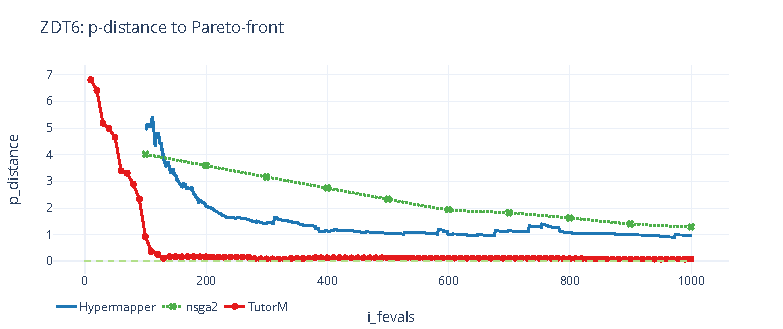
\includegraphics[width=\textwidth]{content/images/zdt6_dist}
                    \caption{Average distance of non-dominant solutions to the real Pareto front}
                    \label{fig:zdt6_dist}
                \end{subfigure} 
                \begin{subfigure}{\textwidth}
                    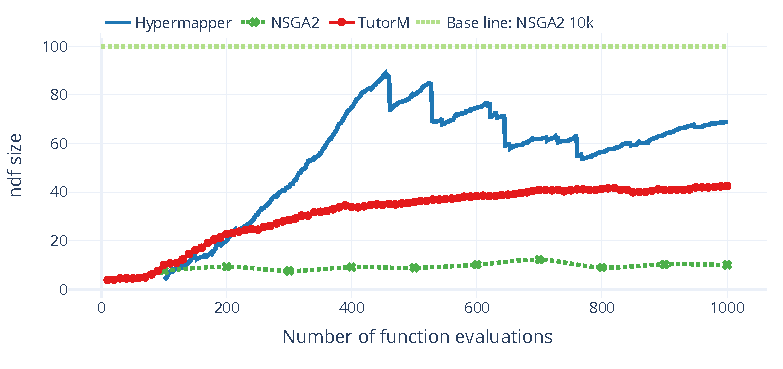
\includegraphics[width=\textwidth]{content/images/zdt6_ndf}
                    \caption{Size of non-dominant solutions across the entire set of the measured solutions}
                    \label{fig:zdt6_ndf}
                \end{subfigure} 

                \begin{subfigure}{\textwidth}
                    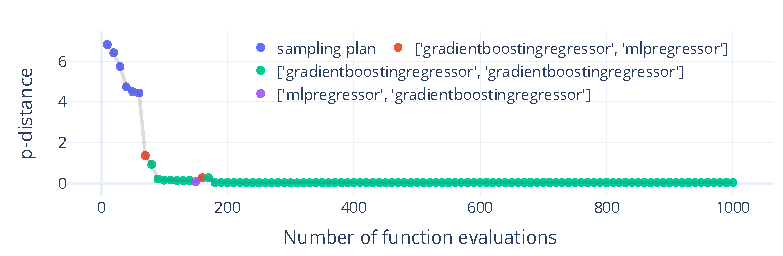
\includegraphics[width=\textwidth]{content/images/zdt6_models}
                    \caption{Best models from the portfolio}
                    \label{fig:zdt6_models}
                \end{subfigure} 

                \caption[Comparison of solutions on ZDT6 problem]{A complex comparison of solutions on ZDT6 problem. Final non-dominated points are used to estimate Pareto-optimal solutions.}
                \label{fig:zdt6_runtime}    
            \end{figure}
    % .... 
    During the first six optimization iterations were used sampling plan until a valid model appeared. This suggests that for a given problem with this surrogate portfolio, the 60 obtained samples from the sampling plan is enough to begin the optimization process. As can be noted, for this problem and with this portfolio, the most suitable compositional surrogate is a \emph{Gradient Boosting Regressor}. 
    
            % ===================== ZDT6: Front
            \begin{figure}
                \centering   
                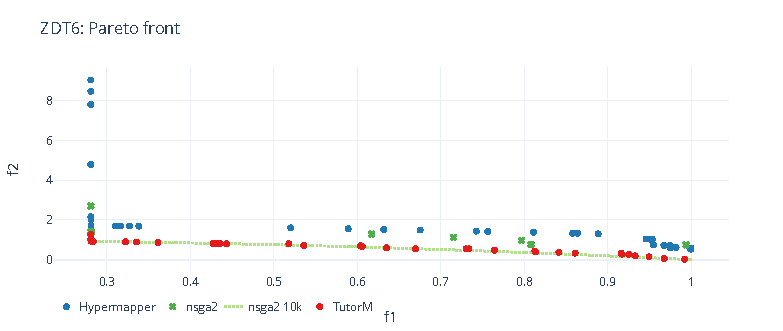
\includegraphics[width=\textwidth]{content/images/zdt6_front}
                \caption[The final assumption of the Pareto optimal solutions (1000 fevals) for ZDT6]{The final assumption of the Pareto optimal solutions (1000 fevals) for ZDT6}
                \label{fig:zdt6_front}
            \end{figure}

	As for NSGA2, the consistently low number of non-dominant solutions explains the slow convergence to the Pareto Front. Above mentioned figures show the values that  NSGA2 reach after 10k function evaluations.
    % The surrogate model can significantly accelerate the ascent to the global optimum. 
    Let's take a look at TutorM and the validation results of the surrogate portfolio. As can be seen in Figure \ref{fig:zdt6_models}, there is an example of a sampling plan and three different compositional surrogate models. The final solution consists of found non-dominant configurations that give an idea of the Pareto Front. From overall Pareto front approximations (Figure \ref{fig:zdt6_front})) only TutorM solutions match with the baseline(NSGA2 10k) while other solutions are close and distributed (Hypermapper) or far away and clustered (NSGA2).

    % ----------------------------------------------------------- Case study's overview
    \subsection*{Case studies: WFG1, WFG4, DTLZ4}
    Below, we compare how optimization process vary across several problems.

    The key feature of the developed method is the dynamic sampling plan, which depends on the quality of available surrogates. 
    As mentioned before, in Figure \ref{fig:zdt6_models}, while the static number of random samples is estimated, it is possible to make optimal decisions much earlier. This approach is applied in TutorM for all optimization problems. By interpreting the end of the sampling plan and the availability of valid models, we can estimate the cross-grain complexity of the unknown problem. From Figure \ref{fig:changing_models} it can be seen a difference in the adaptation of initial samples to problems (WFG1, DTLZ4) and a corresponding improvement in hypervolume. In the case of WFG1, the valid model obtained quickly and reduced initial samplings that may indicate a convenient and unimodal optimization landscape. On the contrary use-case of DTLZ4, sampling plan lasted longer and alternated with valid models. This may indicate the complexity of the problem, such as the multimodality or bias of the landscape. It should also be noted that in each considered case, the best surrogate model is different and may change during optimization. Thus, for the case of DTLZ4, a clear advantage is observed in the choice of composite surrogacy with \emph{Gradient Boosting Regressor}, whereas for WFG1, the multi-objective \emph{Gaussian Process Regressor} is the preferred choice.
    % === TutorM: surrogate portfolio in action
    \begin{figure}
        \centering
        \begin{subfigure}{\textwidth}
            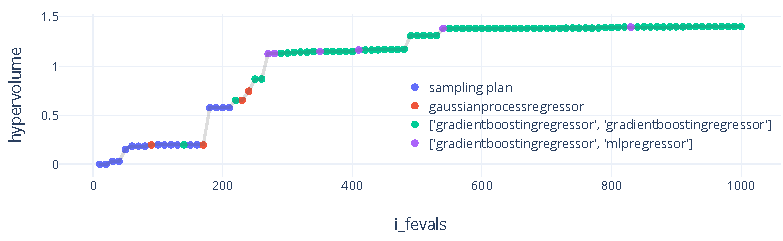
\includegraphics[width=\textwidth]{content/images/dtlz4_models}
            \caption{DTLZ4: sampling plan to the 210th configuration}
            \label{fig:dtlz4_models_210}
        \end{subfigure}
        % \hfill
        
        \begin{subfigure}{\textwidth}
            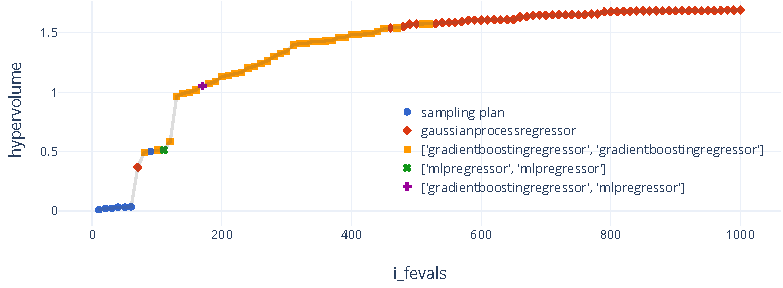
\includegraphics[width=\textwidth]{content/images/wfg1_models}
            \caption{WFG1: sampling plan to the 60th configuration}
            \label{fig:wfg1_models_60}
        \end{subfigure} 

        \caption[Optimization process with dynamic sampling plan and surrogate portfolio.]{Optimization process with dynamic sampling plan and surrogate portfolio. Plots are shown in which step sampling plan was used or which model gives the best accuracy on the test set. Order of the models in the composite surrogates corresponds to the order of the optimization objectives that this model extrapolate.}
        \label{fig:changing_models}    
    \end{figure}


    % For a satisfactory result, the surrogate model needs to describe the overall landscape and the optimization target area. Figure \ref{fig:wfg_14} shows an example of a case where TutorM produces a better or identical result than an optimal solution. The characteristic of this optimization problem lay in flat landscape regions and relative significance of different parameters that significantly impairs the convergence to the global Pareto-optimal solutions. Hypermapper increase count of non-dominated points, regardless it is local optimum and most samples stack in a small region. NSGA2 after 1000 function evaluations also have high-density regions which could be improved with spending more effort to evaluations. The TutorM found several dozen of Pareto-optimal points, that significantly outperforms Hypermapper and even NSGA2 with 10k evaluations. 
    % From WFG4 use case, all over all approaches gain near-optimal results (Fig.\ref{fig:wfg4_front}), but significant advantage over TutorM as it provides an extensive set of solutions (Fig.\ref{fig:wfg4_ndf}) that are well distributed at the Pareto front. As you can see from the graph that the size of the solution increases linearly, which means that effort is spent on improving distribution of the Pareto Pare optimal solutions.

    In the next comparison, we look at WFG1 and WFG4. Figure \ref{fig:wfg14} illustrates how the evaluation budget can be spent to find Pareto optimal solutions. Let's look at the WFG1 (Figure \ref{fig:wfg1_ndf}, \ref{fig:wfg1_front}). It can be seen that TutorM slowly increases the number of solutions during optimization (\ref{sub@fig:wfg1_ndf}). Furthermore, the final result even exceeds the solutions given by the NSGA after 10 thousand function evaluations (\ref{sub@fig:wfg1_front}). With a focus on Hypermapper, the non-dominated plot is highly serrated that indicates that the approach falls within the local optima \ref{sub@fig:wfg1_ndf}. Additional information is revealed from the final Figure \ref{fig:wfg1_front} showed that most final Hypermapper solution strongly clustered, which is lied to wasting of resources.

    For WFG4 use case, all approaches produce near-optimal solutions, but only TutorM provides such an extensive set of solutions(400 from 1000). This means that the optimization process can stop earlier and save the evaluation budget.


    % As shown in Figure \ref{fig:wfg_14}, TutorM could also outperform the MOEA baseline in 10k evaluations(\ref{sub@fig:wfg1_front}). WFG1 has flat landscape regions hence the convergence of genetic algorithms significantly deteriorates. Hypermapper increase count of non-dominated points, regardless it is local optimum and most samples stack in a small region. Nsga2 after 1000 function evaluations also have high-density regions which could be improved with spending more effort to evaluations. The TutorM has several dozen of Pareto-optimal points from all over the budget, that significantly outperforms Hypermapper and nsga2 even with 10k evaluations. 
    % From WFG4 use case, all over all approaches gain near-optimal results(\ref{fig:wfg4_front}), but significant advantage over TutorM as it provides an extensive set of points(\ref{fig:wfg4_ndf}) that are well distributed at the Pareto front.

    % === WFG1 and WFG4
    \begin{figure}
        \centering
        \begin{subfigure}{\textwidth}
            \begin{subfigure}{0.5\textwidth}
                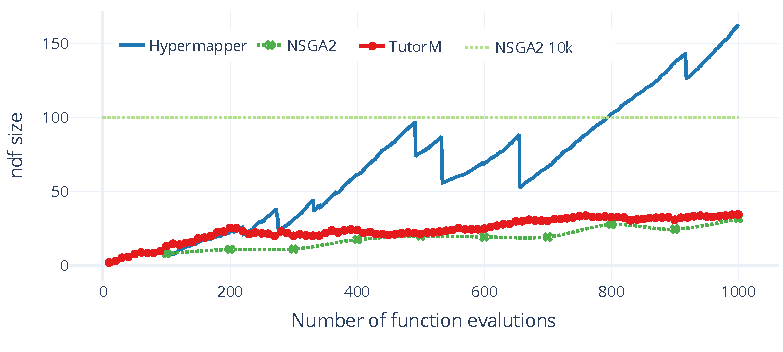
\includegraphics[width=\textwidth]{content/images/wfg1_ndf}
                \caption{WFG1: Size of a non-dominated subset of an evaluated examples}
                \label{fig:wfg1_ndf}
            \end{subfigure} 
            \begin{subfigure}{0.5\textwidth}
                \includegraphics[width=\textwidth]{content/images/wfg1_front}
                \caption{WFG1: Pareto-front approximation}
                \label{fig:wfg1_front}
            \end{subfigure} 
        \end{subfigure} 
        \begin{subfigure}{\textwidth}
            \begin{subfigure}{0.5\textwidth}
                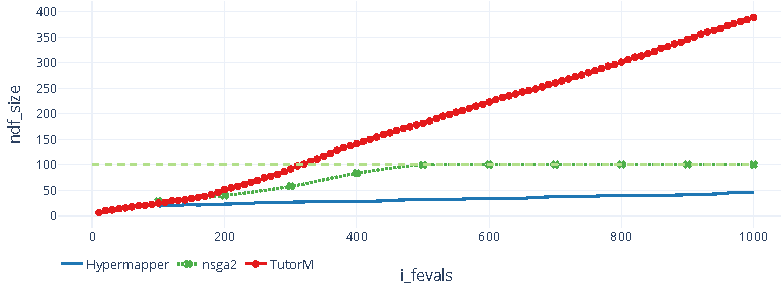
\includegraphics[width=\textwidth]{content/images/wfg4_ndf}
                \caption{WFG4: Size of a non-dominated subset of an evaluated examples}
                \label{fig:wfg4_ndf}
            \end{subfigure} 
            \begin{subfigure}{0.5\textwidth}
                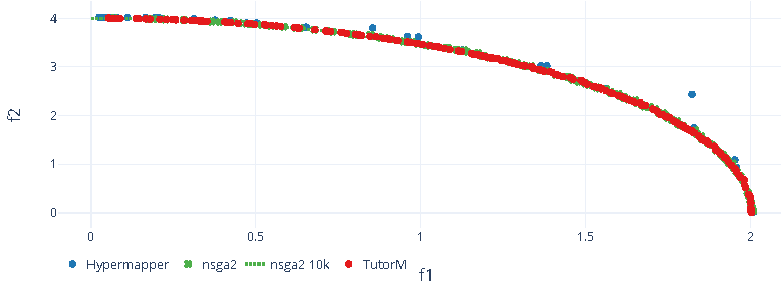
\includegraphics[width=\textwidth]{content/images/wfg4_front}
                \caption{WFG4: Pareto-front approximation}
                \label{fig:wfg4_front}
            \end{subfigure}
        \end{subfigure} 
        \caption[Comparison of solutions on ZDT6 problem]{A complex comparison of solutions on ZDT6 problem. Final non-dominated points are used to estimate Pareto-optimal solutions.}
        \label{fig:wfg14}    
    \end{figure}

% ---------------------------------------------------------- Results
    \subsection*{Results}

    In this benchmark, we analyzed 21 problems from three test sets. They have 2 (3) parameters and 2 objectives. All the experiments were repeated 5 times and averaged. We consider the following metrics:
    \begin{itemize}
        \item \textbf{Hypervolume} This metric is calculated for each comparison because the hypervolume requires a single reference point for a group of competitors. The metric is given as a percentage where $100\%$ corresponds to the maximum volume in competition and $0\%$ corresponds to the hypervolume of a random set of solutions.
        \item \textbf{p-distance} The primary metric for evaluation. Unfortunately, not available for WFG problems.
        \item \textbf{non-dominated font(ndf) size} The ratio of the number of final non-dominated decisions to the number of spent function evaluations.
        \item \textbf{Spacing} The inverse spacing metric is calculated, where 1 corresponds to the most cohesive decisions among competitors.
    \end{itemize}

    In Table \ref{tab:magic_five}, we present a subgroup of problems that have varying complexity. The full list of results is provided in the appendix (\hyperref[tab:zdt_summary]{ZDT}, \hyperref[tab:dtlz_summary]{DTLZ}, \hyperref[tab:wfg_summary]{WFG}).

        % Please add the following required packages to your document preamble:
    % \usepackage{booktabs}
    % \usepackage{multirow}
    \begin{table}[]
        \centering
        \caption{Comparison of final results after 1000 function evaluations}
        \begin{tabular}{@{}lllllll@{}}
        \toprule
                                                                                                & Metric        & ZDT4             & ZDT6             & DTLZ4             & WFG1             & WFG4             \\ \midrule
        \multirow{4}{*}{\textbf{TutorM}}                                                          & Hypervolume   & \textbf{99,80\%} & \textbf{99,43\%} & \textbf{99,829\%} & \textbf{95,75\%} & \textbf{99,28\%} \\ \cmidrule(l){2-7} 
                                                                                                & p-distance    & \textbf{0,01}    & \textbf{0,09}    & \textbf{0,001}    & -                & -                \\ \cmidrule(l){2-7} 
                                                                                                & ndf-size      & \textbf{50,0\%}  & 4,26\%           & 0,2\%             & 3,44\%           & \textbf{38,90\%} \\ \cmidrule(l){2-7} 
                                                                                                & space-metric  & \textbf{0,78}    & 0,17             & 0,666             & 0,51             & \textbf{1}       \\ \midrule
        \multirow{4}{*}{\textbf{NSGA2}}                                                           & Hypervolume   & 83,43\%          & 83,84\%          & 87,807\%          & 30,52\%          & 83,95\%          \\ \cmidrule(l){2-7} 
                                                                                                & p-distance    & 0,04             & 1,29             & 0,002             & -                & -                \\ \cmidrule(l){2-7} 
                                                                                                & ndf-size      & 8,77\%           & 1,01\%           & 9,600\%           & 3,18\%           & 10\%             \\ \cmidrule(l){2-7} 
                                                                                                & space-metric  & 0,19             & 0,04             & 0,323             & 0,28             & 0,58             \\ \midrule
        \multirow{4}{*}{\textbf{Hypermaper}}                                                      & Hypervolume   & 97,32\%          & 82,86\%          & 64,57\%           & 44,12\%          & 84,39\%          \\ \cmidrule(l){2-7} 
                                                                                                & p-distance    & 0,90             & 1,12             & 0,059             & -                & -                \\ \cmidrule(l){2-7} 
                                                                                                & ndf-size      & 5,42\%           & \textbf{6,25\%}  & 1,177\%           & \textbf{10,24\%} & 3,26\%           \\ \cmidrule(l){2-7} 
                                                                                                & space-metrics & 0,11             & 0,08             & 0,029             & 0,31             & 0,06             \\ \midrule
        \multirow{4}{*}{\textbf{\begin{tabular}[c]{@{}l@{}}NSGA2 50k\\ (Base line)\end{tabular}}} & Hypervolume   & 100\%            & 100\%            & 100\%             & 100\%            & 100\%            \\ \cmidrule(l){2-7} 
                                                                                                & p-distance    & 2,04e-05         & 0,0003           & 8,81e-06          & -                & -                \\ \cmidrule(l){2-7} 
                                                                                                & ndf-size      & 0,72\%           & 0,72\%           & 0,360\%           & 0,72\%           & 0,72\%           \\ \cmidrule(l){2-7} 
                                                                                                & space-metric  & 1                & 1                & 1                 & 1                & 0,60             \\ \bottomrule
        \end{tabular}
        \label{tab:magic_five}
    \end{table}




        % \begin{table}[]
    %     \centering
    %     \caption{Comparison of final results after 1000 feature evaluations}
    %     \resizebox{\textwidth}{!}{%
    %     \begin{tabular}{@{}ccccccc@{}}
    %     \toprule
    %                                          & \textbf{Metric}        & \textbf{ZDT4} & \textbf{ZDT6} & \textbf{DTLZ4} & \textbf{WFG1} & \textbf{WFG4} \\ \midrule
    %     \multirow{4}{*}{\textbf{TutorM}}     & \textbf{hypervolume}   & 99,45\%       & 99,01\%       & 99,27\%        & 115,60\%      & 95,95\%       \\
    %                                          & \textbf{p-distance}    & 1,336         & 0,522         & 0,022          & -             & -             \\
    %                                          & \textbf{ndf-size}      & 183,022       & 31,528        & 119,308        & 24,158        & 183,244       \\
    %                                          & \textbf{space-metrics} & 0,103         & 0,142         & 0,186          & 0,129         & 0,032         \\ \midrule
    %     \multirow{4}{*}{\textbf{NSGA2}}      & \textbf{hypervolume}   & 97,57\%       & 87,46\%       & 95,87\%        & 45,01\%       & 91,87\%       \\
    %                                          & \textbf{p-distance}    & 1,391         & 1,872         & 0,022          & -             & -             \\
    %                                          & \textbf{ndf-size}      & 44,000        & 11,455        & 39,900         & 20,164        & 82,436        \\
    %                                          & \textbf{space-metrics} & 0,176         & 0,355         & 0,268          & 0,228         & 0,038         \\ \midrule
    %     \multirow{4}{*}{\textbf{Hypermaper}} & \textbf{hypervolume}   & 96,82\%       & 66,95\%       & 81,29\%        & 40,66\%       & 74,09\%       \\
    %                                          & \textbf{p-distance}    & 2,024         & 1,850         & 0,076          & -             & -             \\
    %                                          & \textbf{ndf-size}      & 28,908        & 52,746        & 10,743         & 81,512        & 30,158        \\
    %                                          & \textbf{space-metrics} & 0,1386        & 0,11621       & 0,5282         & 0,0870        & 0,1032        \\ \midrule
    %     \multirow{4}{*}{\textbf{\begin{tabular}[c]{@{}c@{}}NSGA2\\ 10k eval\end{tabular}}} & \textbf{hypervolume}      & 100,00\% & 100,00\% & 100,00\% & 100,00\% & 100,00\% \\
    %                                          & \textbf{p-distance}    & 0,152         & 0,256         & 0,002          & -             & -             \\
    %                                          & \textbf{ndf-size}      & 93,901        & 79,776        & 93,990         & 85,196        & 98,087        \\
    %                                          & \textbf{space-metrics} & 0,033         & 0,074         & 0,039          & 0,051         & 0,016         \\ \bottomrule
    %     \end{tabular}%
    %     }
    % \label{tab:magic_five} 
    % \end{table}

    Therefore, from the obtained results, it follows that the developed strategy generally gives optimal or better results than the baseline on most of the investigated problems. 

    We assume that good results are predetermined by new features such as surrogate models portfolio and adaptive sampling plan. These features have yielded significant results on almost all problems. However, we did not apply inner parameter tuning: in all experiments, TutorM was used with default parameters.

% --------------------------------------------------------------------------------------------
% ---------------------       Benchmark 2: Dynamic sampling plan and parameter selection
% --------------------------------------------------------------------------------------------
\section{Benchmark 2: Inner parameters} \label{sec:bench2}
    In this benchmark, we investigate whether it is possible to further improve the performance of TutorM by tuning its parameters. We examine the effect of internal parameters on the performance and quality of optimization. As was mentions, in the previous section, it was applied with a default setting. 

    \subsection{TutorM parameters}
    Besides the standard model-based parameters, it is necessary to investigate the impact of additional TutorM parameters such as validation thresholds, test set size and prediction size. This research is needed to select the optimal configuration that can significantly improve the result of the existing system. Unfortunately, there is not enough information about how to configure the model-based parameter optimization \cite{TobiasCV, HybridSurrRCG}. Conducting such analysis is useful not only for the availability of the TutorM but also for the general tuning of model-based optimization.  
    Due to limited time, we consider only the ZDT4 and ZDT6 problems with a surrogate portfolio from the previous benchmark, but without the \emph{Gaussian regression model}. This model takes a long time to train and the full factorial design does not fit within our time frame.
    % Secondly, hyperparameter tuning for a spe- cific model class, selecting from a finite amount of different models and possibly choosing relevant features are important steps in practical optimization. It

    The following parameters are exposed in the developed TutorM class:
    \begin{itemize}
        \item \textbf{Initial dataset} [\underline{0}, 100, 500, 750]. The initial number of points obtained from sampling plan. At the same time, the total budget for measurements remains unchanged and equals 1000. Default value is 0.
        \item \textbf{Surrogate validation.} Criteria and parameters for evaluating the usefulness of the surrogate model.
            \begin{itemize}
                \item \textbf{Train/test split} [\underline{75/25}, 90/10] splitting proportion in which the available samples for training and testing is divided. Train and test sets are crucial to ensure that the surrogate model is able to generalize well to new data. Default value is 75/25
                \item \textbf{Cross-validation threshold}[0.2, \underline{0.65}, 0.9] minimum accuracy threshold for any round in cross-validation(CV). CV is used to select valid surrogate models and avoid overfitting. Default values is 0.65
                \item \textbf{Test threshold} [0, \underline{0.6}, 0.9] minimum accuracy threshold on the test set. The accuracy obtained from the test set and is used to verify valid models of how they extrapolate unknown data. Default values is 0.6
            \end{itemize}
        \item \textbf{Optimization search algorithm} [NSGA2, \underline{MOEA-Ctrl}] optimization algorithm for multi-objective solutions. Default value is MOEA-Ctrl.
        \item \textbf{Solution combinations} [Non-dominated front score(ndf score), \underline{Stacking}] approach for choosing a set of solutions from a valid surrogate model. Since several models can be valid and each one provides its own set of decisions, we have to choose which one to pick. \emph{Non-dominated front score (ndf score)} prefers the surrogate model with the highest precision for non-dominant solutions, whereas the \emph{stack} integrates all available surrogate solutions into one set of solutions. Default value is Stack.
        \item \textbf{Prediction count} [\underline{10}, 100] number of random solutions for a real evaluation that are selected from the set of solutions. Default value is 10.
    \end{itemize}

    As a result of a full factorial design, 576 possible combinations were obtained. Each combination was repeated 5 times and averaged. Conclusions were made on the selected 40 best and worst combinations.

    % ---------------------------------------------- ZDT6
    First, let's consider the ZDT6 problem. Inspection of Figure \ref{fig:conf_zdt6} indicates that the \emph{solution combination} made the most significant impact on the result.  There is a definite advantage in combining solutions into a stack. The second important parameter is the \emph{Optimization search algorithm}(Solver). The best configurations prefer to pick a combination of Genetic Algorithms (MOEA-Ctrl) as the optimization solver.

        % ===  ------------------------------------- ZDT6
        \begin{figure}
            \centering
            \begin{subfigure}{\textwidth}
                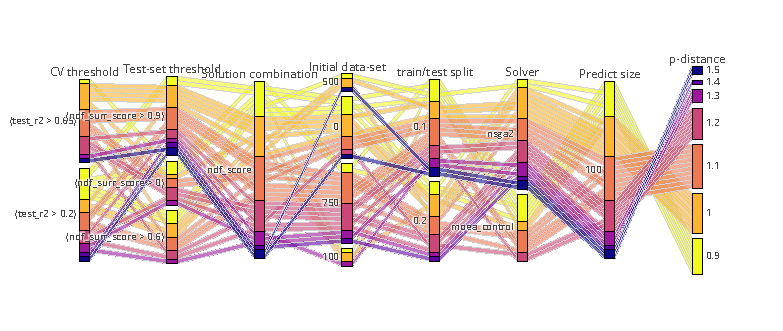
\includegraphics[width=\textwidth]{content/images/conf_zdt6_worst}
                \caption{40 worst configurations}
                \label{fig:conf_zdt6_worst}
            \end{subfigure} 
            % \hfill
            
            \begin{subfigure}{\textwidth}
                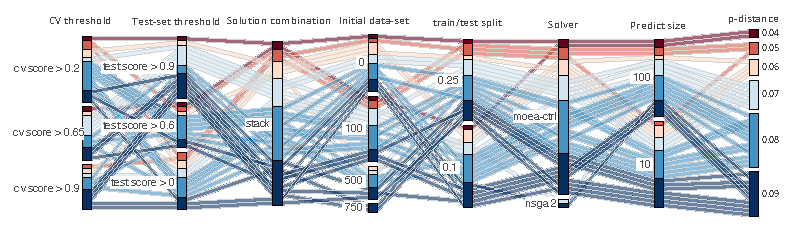
\includegraphics[width=\textwidth]{content/images/conf_zdt6_best}
                \caption{40 best configurations}
                \label{fig:conf_zdt6_best}
            \end{subfigure}   
            \caption[ZDT6: The selection from average result of best and worst configurations.]{ZDT6: The selection from average result of best and worst configurations.}
            \label{fig:conf_zdt6}    
        \end{figure}
    
    Let us look at the \emph{solution combination} and the \emph{Optimization search algorithm} options in more details (Fig. \ref{fig:conf_zdt6_sign}). The impact of changing the optimization solver is highly dependent on the solution combination strategy. Improvement in result for MOEA-Ctrl solver is more significant when their results are combined into a stack. This advantage can be explained by the fact that the stack reduces the bias of surrogate models while the combination of genetic algorithms decreases prediction variance.

        % === ZDT 6
        \begin{figure}
            \centering
            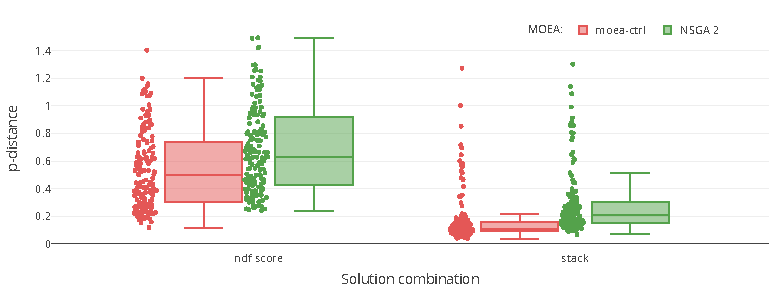
\includegraphics[width=0.8\textwidth]{content/images/conf_zdt6_solver}
            \caption[Correlation between the most influenceable parameters for the ZDT6]{Correlation between the most influenceable parameters for the ZDT6: solution combination strategy and optimization algorithm}
            \label{fig:conf_zdt6_sign}    
        \end{figure}

    % ---------------------------------------------- ZDT4
    Now let us look at the ZDT4 problem (Fig. \ref{fig:conf_zdt4}). The results are similar to those obtained with the ZDT6 problem: the solutions stack take part almost in all best configurations. However, in this problem, there is no clear dominance of an optimization solver, but there is an impact on results from the validation thresholds (Figure \ref{fig:conf_zdt4_sign}). 
    A significant difference is available for the cross-validation threshold in the case of \textit{ndf score} \emph{solution combination} set (Figure \ref{fig:conf_zdt4_worst}). It should be noted that the stack makes the validation threshold impact less significant as evident from the Figure \ref{fig:conf_zdt4_sign}. This influence is related to the general characteristics of this technique to reduce the bias of solutions.
        % === -------------------------------------- ZDT 4
        \begin{figure}
            \centering
            \begin{subfigure}{\textwidth}
                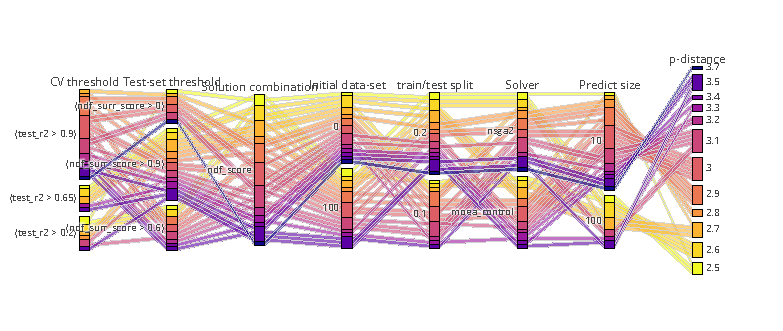
\includegraphics[width=\textwidth]{content/images/conf_zdt4_worst}
                \caption{ZDT4: worst configurations}
                \label{fig:conf_zdt4_worst}
            \end{subfigure} 
            % \hfill       
            \begin{subfigure}{\textwidth}
                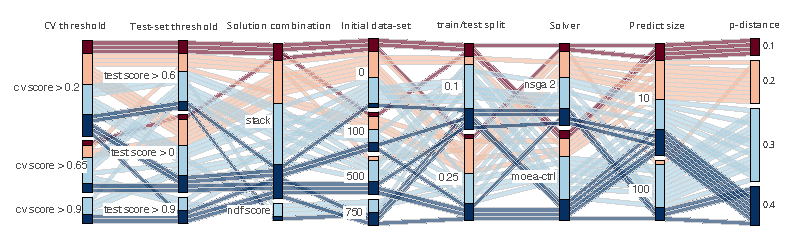
\includegraphics[width=\textwidth]{content/images/conf_zdt4_best}
                \caption{ZDT4: best configurations}
                \label{fig:conf_zdt4_best}
            \end{subfigure} 
    
            \caption[ZDT4: The selection from average result of best and worst configurations.]{ZDT4: The selection from average result of best and worst configurations.}
            \label{fig:conf_zdt4}    
        \end{figure}
    
        % === ZDT4
        \begin{figure}
            \centering
            \begin{subfigure}{\textwidth}
                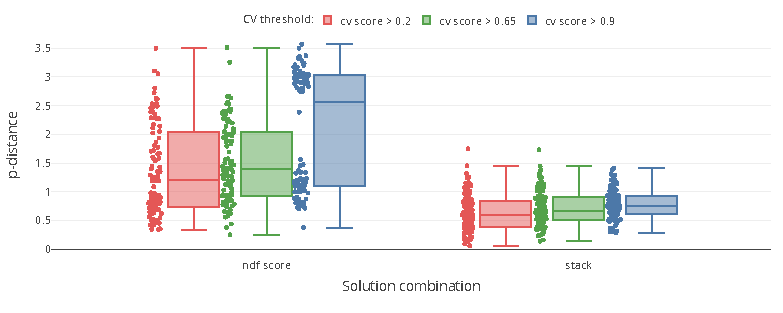
\includegraphics[width=\textwidth]{content/images/conf_zdt4_cv_score}
                \caption{An impact of the cross-validation's threshold}
                \label{fig:zdt4_pred_solver}
            \end{subfigure} 
            \begin{subfigure}{\textwidth}
                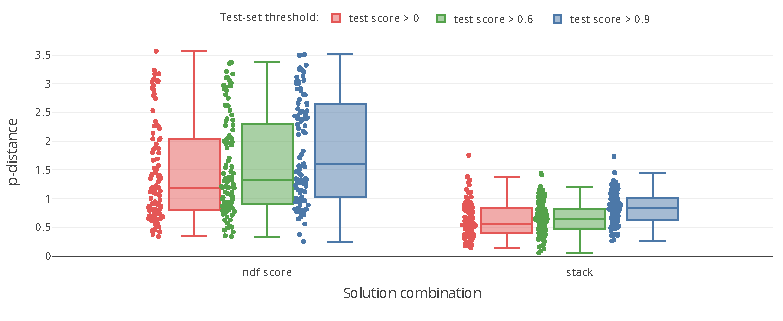
\includegraphics[width=\textwidth]{content/images/conf_zdt4_test_score}
                \caption{An impact of the test-set-validation's threshold}
                \label{fig:zdt4_comb_valid}
            \end{subfigure}
            \caption[Correlation between the most influenceable parameters for the ZDT4]{Correlation between the most influenceable parameters for the ZDT4} 
            \label{fig:conf_zdt4_sign}    
        \end{figure}

    Another interesting conclusion could be done from the \emph{initial sample size}. The worst and the best configurations are most affected by the missing sampling plan. Reason for this is that the small number of samples may lead to a surrogate model fallacy in extrapolation the search space while, at the same time, the small number of samples provide more opportunities for optimization search.

    % ====================================================== Start set for Hypermapper 2.0
    \subsection{Sampling plan size}
    The purpose of this experiment is to review the dependencies between the optimization result and the sampling plan size. The Hypermapper was selected as a foundation for analysis because it has a static implementation of the optimization algorithm with the surrogate model.

    The results are shown in the following Figure \ref{fig:hmapper_start_set}. For WFG problems, the criterion is the hypervolume and for ZDT problems is the p-distance. Of all the results, the initial sampling plan has the smallest effect on the WFG6. Since this problem is unimodal and model require fewer samples for extrapolation. Other problems have a more complicated multimodal landscape that shown by unstable results. 

        \begin{figure}[!h]
            \centering
            \begin{subfigure}{\textwidth}
                \begin{subfigure}{0.45\textwidth}
                    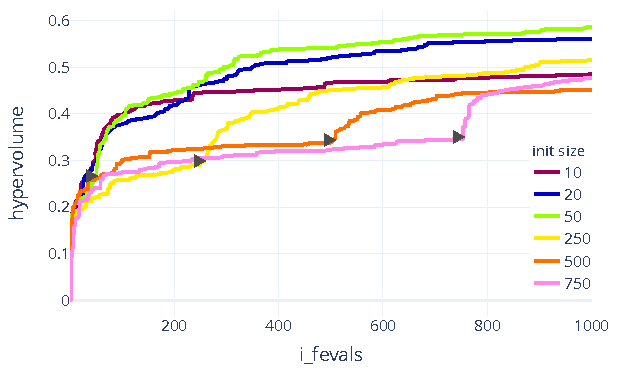
\includegraphics[width=\textwidth]{content/images/hypermapper_wfg1_start_set}
                    \caption{WFG1}
                    \label{fig:hmapper_wfg1_start_set}
                \end{subfigure}
                \begin{subfigure}{0.45\textwidth}
                    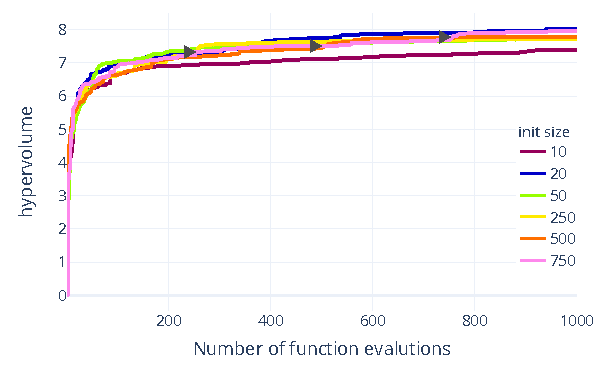
\includegraphics[width=\textwidth]{content/images/hypermapper_wfg4_start_set}
                    \caption{WFG4}
                    \label{fig:hmapper_wfg4_start_set}
                \end{subfigure}
            \end{subfigure} 
            \hfill

            
            \begin{subfigure}{\textwidth}
                \begin{subfigure}{0.45\textwidth}
                    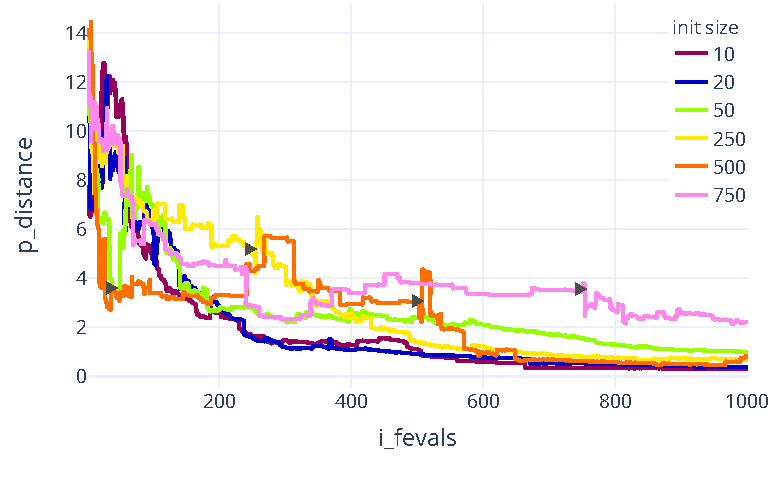
\includegraphics[width=\textwidth]{content/images/hypermapper_zdt4_start_set}
                    \caption{ZDT4}
                    \label{fig:hmapper_zdt4_start_set}
                \end{subfigure}
                \begin{subfigure}{0.45\textwidth}
                    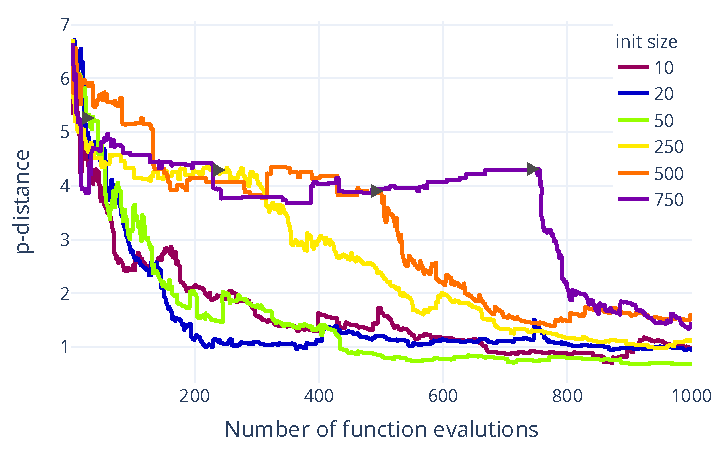
\includegraphics[width=\textwidth]{content/images/hypermapper_zdt6_start_set}
                    \caption{ZDT6}
                    \label{fig:hmapper_zdt6_start_set}
                \end{subfigure}
            \end{subfigure} 

            \caption[Influence of the initial sample plan for optimization with Hypermapper 2.0.]{Influence of the initial sample plan for optimization with Hypermapper 2.0.}
            \label{fig:hmapper_start_set}    
        \end{figure}

    % -------------------------------------------------   Results
    \subsection*{Results}
    We investigate the possible parameters of TutorM and determine which ones allow us to improve results. It was noted that \emph{Solution combinations} and \emph{Optimization search algorithm} had the most significant impact on the quality of the solution. The \emph{stack} of solutions with the combined \gls{ea} algorithms (MOEA-Ctrl) is the best combination of parameters which is the default for TutorM. 
    The other parameters tested have a much smaller effect, indicating that the default TutorM configuration is optimal.


% --------------------------------------------------------------------------------------------
% ---------------------       Benchmark 3: Many-objective optimization, scaling
% --------------------------------------------------------------------------------------------
\section{Benchmark 3: Scalability of surrogate models}
    Not only the type of the problem landscape but also its dimensions is an essential factor for picking the surrogate model. The advantage of a surrogate model might be lost when the number of parameters or criteria are changed. The goal of this experiment is to find out the scalability of surrogate models. 

    The following surrogates were selected for the evaluation:
    \begin{itemize}
        \item \emph{Gaussian Process Regressor} with kernel design from GPML\cite{RasmussenN10}. Gaussian process models are well known and are commonly used in Bayesian optimization for a wide variety of problems \cite{EmmerichGN06, MlakarPTF15}. 
        \item \emph{MLPRegressor} is a neural network implementation from the \textit{sklearn} framework. Neural networks could automatically discover useful representations in high-dimensional data by learning multiple layers \cite{WilsonHSX16}. Because this model simultaneously extrapolates all objectives, we intuitively chose an architecture that consists of 5 layers and 100 neurons per layer.
        \item The surrogate portfolio is included of Gradient Boosting Regressor, MLPRegressor and \emph{SVR (RBF kernel)} as mentioned in Section~\ref{sec:bench2}.
    \end{itemize}

    DTLZ2 problem was selected to evaluate the scalability of the surrogate models. It is a unimodal problem with multiple global optima and concave geometry of the Pareto front. 
    During the experiment on DTLZ2, the number of optimization criteria changes with a constant number of parameters. Figure \ref{fig:scale_dtlz2} shows the three selected surrogate strategies with the average distance to the Pareto front (first row) and a time spent per optimization iteration (bottom row). For all cases, the experiment was repeated 5 times.

        % ------------------ Scale DTLZ 
        \begin{figure}[h]
            \centering
            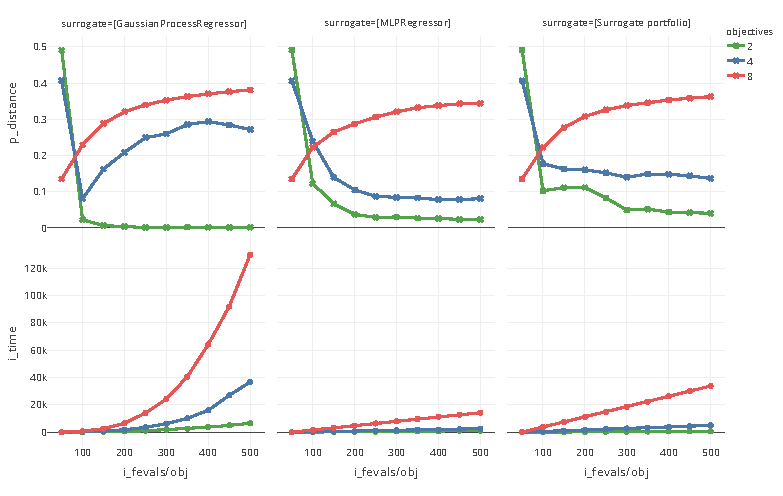
\includegraphics[width=\textwidth]{content/images/scale_dtlz2}
            \caption[Scaling example for the three variants of the surrogate on the DTLZ2.]{Scaling example for the three variants of the surrogate on the DTLZ2  with the 9-dimensional objective space.}
            \label{fig:scale_dtlz2}    
        \end{figure}

    As illustrated by Figure \ref{fig:scale_dtlz2}, \emph{Gaussian Process Regressor} model shows significantly better results relative to other approaches but only for the bi-objective problem. Increase the number of objectives to four, leads to the fact that only the \emph{MLPRegressor} and the surrogate portfolio are converged to an optimal solution. Further increasing the number of objectives follows, then the search space becomes too complicated, and all approaches fail to find solutions.
    
    \subsection*{Results}
    The ability of models to estimate the search space depends on their hyperparameters. As an example: \emph{Gaussian Process Regressor} are highly dependent on the kernel while \emph{MLPRegressor} depends on a number of layers.
    In turn, for the surrogate portfolio, the parameters determine how to \emph{build and select} surrogate models. The same model but with different parameters, is evaluated in the portfolio as separate entities. So, required scalability in solving the multi-dimensional problem could be achieved with scalability that provides surrogate portfolio. 


% --------------------------------------------------------------------------------------------
% ------------------------------------------------     Discussion 
% --------------------------------------------------------------------------------------------
\section{Result discussion}

The purpose of this thesis is to investigate the mechanism of a cross-grained model composition for solving multi-objective problems. In the evaluation, we provide an extensive comparative analysis of developed techniques on a wide range of problems. The analysis also includes exhaustive verification of possible parameters and the impact of the sampling plan. The possibility of scaling surrogate models with increasing the number of objectives was also tested.

From the benchmarks we can draw the following conclusions:
\begin{enumerate}
    \item The developed method(TutorM) is far ahead of the considered analogues and achieves optimum result with a considerable saving of functional evaluations. In some cases, the results obtained with TutorM are better than the selected baseline.
    \item Parameter studies for TutorM have shown that a significant result improvement is achieved by combining solutions with multiple surrogates (solution stack).
    \item The possibilities of scaling up the surrogate portfolio were tested. The results show that the dynamic selecting surrogate model with the variation for specific dimensionality of the problem is essential.
\end{enumerate}




% consume an inordinate amount of time.


% The purpose of this work is to explore the possibility of using single-objective models for many-objective optimizations. To accomplish this goal, the composite model has been implemented. It is used to combine models into a portfolio and dynamically select them. Furthermore, the stepwise validation approach has been adapted to evaluate the usability of the surrogate model.


% Up to now, most papers used the The quality of the results obtained with X was similar to the results obtained with Y, but with significantly fewer exactly evaluated solutions during the optimization process. 


% Discussion

% non-separable
% or have a deceptive fitness landscape

% However, GAs, or at least some variants of them, are not 100'\%' ruled out.

% +’, ’−’ and ’≈’, which indicate that the result is significantly better, significantly worst and statistically similar to the result in the control column, respectively. 


% On the left side the learning curve of a naive Bayes classifier is shown for the digits dataset. Note that the training score and the cross-validation score are both not very good at the end. However, the shape of the curve can be found in more complex datasets very often: the training score is very high at the beginning and decreases and the cross-validation score is very low at the beginning and increases. On the right side we see the learning curve of an SVM with RBF kernel. We can see clearly that the training score is still around the maximum and the validation score could be increased with more training samples.
% https://scikit-learn.org/0.15/auto_examples/plot_learning_curve.html




% Compared to Auto-WEKA, this is much more data-efficient: in
% Auto-WEKA, evaluating the performance of an ensemble with 5 components requires the construction
% and evaluation of 5 models; in contrast, in auto-sklearn, ensembles come largely for free, and it is
% possible to mix and match models evaluated at arbitrary times during the optimization.


% This makes the archive gradually move towards the Pareto-front.
% 80% of the computing-time is spent in the area close to the Pareto front.


% We would like to prove that the use of hierarchical surrogates has a higher probability to find the optimum of the optimization problem in Eq. (4) ref[Evolutionary optimization with hierarchical surrogates]


% Test problems ZDT1, ZDT2, and ZDT3 show a different trend in function evaluations as compared to OSY.


% In contrast to PR, ANN, RBF, GP, Ranking SVM is invariant to

% The measurements were performed on an Intel Core i7-8700CPU machine with 64G of memory using Fedora Server 29.
